\section{CutMix}

CutMix, iki görüntüyü birleştirerek sınıflandırma modellerini daha güçlü ve yerelleştirilebilir özellikler öğrenmeye teşvik eder. CutMix, iki görüntüyü kesip birleştirerek yeni bir görüntü oluşturur ve aynı zamanda sınıf etiketlerini de karıştırır. Böylece model, görüntünün hem görsel hem de sınıfsal olarak farklı alanlarına odaklanmaya zorlanır. CutMix, iki görüntü seçer ve birincisinden rastgele bir bölgeyi alır, ardından bu bölgeyi ikinci görüntüye yerleştirir. Görüntüler karıştırılırken sınıf etiketleri de orantılı olarak karıştırılır. Bu, modelin farklı sınıf etiketlerini öğrenmesine ve bu etiketlerin hangi görüntü alanlarıyla ilişkili olduğunu anlamasına yardımcı olu

\subsubsection{Python Kodu}

\begin{lstlisting}[language=Python]
from art.defences.preprocessor import CutMixTensorFlowV2

cutmix = CutMixTensorFlowV2(num_classes=10, apply_fit=True, apply_predict=False)
cutmix_train = cutmix.forward(x=x_train, y=y_train)
\end{lstlisting}

\begin{figure}[h]
    \centering
    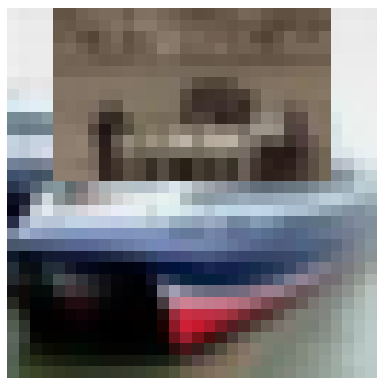
\includegraphics[width=0.4\textwidth]{images/cutmix_example.png}
    \caption{}
\end{figure}

\newpage